\chapter{Métodos}\label{chapter:Metodos}
En este capítulo se detallan los criterios seguidos para la elección de la geometría de los espaciadores y su escala, los cálculos realizados para adaptar las propiedades de los materiales a las limitaciones de escala de los programas de simulación, los procedimientos seguidos para realizar las simulaciones y el procedimiento seguido para la extracción de los datos de la simulación de CFD.
\section{Criterios de geometría y escala}
Los criterios de geometría y escala se basan principalmente en el proceso de fabricación de los nano-espaciadores por fotolitografía, que es la técnica que se utilizará en el desarrollo de los primeros experimentos que intentarán corroborar los resultados obtenidos en este trabajo de simulación, esto en una siguiente etapa de la investigación.\\\\
La base del nano-espaciador es cuadrada por ser la geometría más sencilla de fabricar mediante procesos fotolitográficos y para realizar cálculos, por ser sus ecuaciones de área y volumen las más sencilla de los polígonos regulares cerrados. El lado de la base del nano-espaciador son de 3 $\mu m$ por ser el límite de resolución de la mayoría de equipos de fotolitografía, es decir, es la mínima distancia que se puede definir mediante fotolitografía.\\\\
Se utiliza 100 nm como la distancia mínima para definir la altura mínima de los nano-espaciadores, correspondiente a 1 mm de la escala del modelo 3D en Inventor. Por lo tanto, el factor de escala que se aplica a las unidades de longitud es $10^4$, que se toma en cuenta a la hora de definir las propiedades térmicas que involucren unidades de longitud, como es la conductividad térmica ($W/m2$).
%%% CALCULOS DE LAS PROPIEDADES DE LOS MATERIALES
\section{Cálculos de las propiedades de los materiales para las simulaciones}
Para obtener los nuevos parámetros de distancias, áreas y volúmenes del modelo 3D del nano-espaciador se procede a obtener las relaciones de escala entre el modelo y la realidad. También se obtienen las relaciones de las propiedades más significativas de los materiales de la realidad y las simulaciones de transmisión de calor por conducción, siendo la principal propiedad la conductividad térmica. Otras propiedades que se toman en cuenta son la densidad y el calor específico, teniendo que destacar la resistencia de contacto por unidad de área entre el nano-espaciador y el emisor.\\\\
Para diferenciar las dimensiones reales de las dimensiones utilizadas en el modelo 3D se utilizará el apostrofe después de la variable correspondiente, por ejemplo, para la longitud real se usa $L$ y para la longitud en el modelo 3D se usa $L'$.\\\\
La relación de longitudes entre el modelo 3D y la realidad es:
\begin{equation}
{L'}/{L}={1mm}/{100nm}=10^4
\label{eq:relacion_longitud}
\end{equation}
%%%  AREA
\subsection{Área}
La sección de los nano-espaciadores es un cuadrado cuya fórmula de área es $A=L^2$, donde $A$ es el área y $L$ el lado del cuadrado, siendo la relación de las áreas la siguiente:
\begin{equation}
	\dfrac{A'}{A}=\left(\dfrac{L'}{L}\right)^2=10^8
	\label{eq:relacion_areas}
\end{equation}
%%% VOLUMEN
\subsection{Volumen}
El volumen de un prisma de base cuadrada se expresa como $V=A\cdot L$, donde $L$ es la altura del prisma.
\begin{equation}
	\dfrac{V'}{V}=\dfrac{A'\cdot L'}{A\cdot L} = 
	\dfrac{A'}{A}\cdot \dfrac{L'}{L} \ \Longrightarrow \ \dfrac{V'}{V} =10^{12}
	\label{eq:relacion_volumen}
\end{equation}
El volumen de cada nano-espaciador en el modelo será $10^{12}$ veces el volumen original.
%%% DENSIDAD
\subsection{Densidad}
La masa de cada elemento es igual entre el modelo($M'$) y la realidad($M$), por lo tanto la densidad varía.
\begin{equation}
\dfrac{\rho '}{\rho}=\dfrac{M'/V'}{M/V}=\dfrac{M'}{M}\cdot \dfrac{V}{V'} \ \Longrightarrow \ 
\dfrac{\rho '}{\rho}=10^{-12}
\label{eq:relacion_densidad}
\end{equation}
La densidad de cada elemento en el modelo será $10^{-12}$ veces la densidad de la realidad.
%%% CONDUCTIVIDAD TERMICA
\subsection{Conductividad Térmica}
La resistencia térmica de los materiales del modelo de simulación se mantiene igual a la de la realidad, por lo tanto, la conductividad térmica de los materiales en el modelo son distintas a la realidad. Sabiendo que la fórmula de la resistencia térmica de conducción es $R=1/k \cdot L/A$, donde $k$ es la conductividad térmica, $L$ la longitud y $A$ es la sección, se puede obtener la relación de las conductividades térmicas del modelo de simulación respecto a la realidad.
\[ \dfrac{R}{R'}= \dfrac{1/k}{1/k'}\cdot \dfrac{L/A}{L'/A'}= \dfrac{k'}{k}\cdot \dfrac{L}{L'}\cdot \dfrac{A'}{A}=1\]
\begin{equation}
\dfrac{k'}{k}=\dfrac{L'}{L}\cdot \dfrac{A}{A'}=\dfrac{10^4}{10^8} \ \Longrightarrow \ \dfrac{k'}{k}=10^{-4}
\label{eq:relacion_conductividadTermica}
\end{equation}
Para el caso del nano-espaciador de $SiO_2$ que puede presentar diferentes porosidades para el material, se multiplica la conductividad térmica por la conductividad térmica normalizada para dicha porosidad \cite{ThermalConductivity_SiO2_2018}.
%%% CALOR ESPECIFICO
\subsection{Calor Específico}
El calor específico de los materiales del modelo de simulación es el mismo que el de la realidad porque el calor específico se define como la cantidad de calor necesaria que hay que suministrar a una unidad de masa para elevar su temperatura en una unidad, como la masa del modelo de simulación es igual a la de la realidad, la cantidad de energía necesaria para elevar una unidad de temperatura va a ser igual al del modelo de simulación respecto a la realidad, por lo tanto, el calor específico se mantiene igual al de la realidad.
%%% RESISTENCIA DE CONTACTO
\subsection{Resistencia de contacto}\label{sec:metodos_Rc}
La resistencia de contacto ($R_c$) es difícil de modelar matemáticamente en una ecuación ya que depende de muchas variables, como la temperatura, presión, entre otros. La resistencia de térmica producida por la resistencia de contacto es $R_{th}=R_{c}/A$, donde A es la superficie de contacto, por lo tanto se ve afectado por la diferencia de escala entre el modelo de simulación y la realidad.
\[ \dfrac{R_{th}'}{R_{th}}=\dfrac{R_c'}{R_c}\cdot \dfrac{A}{A'}=1 \]
\begin{equation}
	\dfrac{R_{th}'}{R_{th}}=\dfrac{R_c'}{R_c}\cdot \dfrac{A}{A'}=1 \ \Longrightarrow \  \dfrac{R_c'}{R_c}=\dfrac{A'}{A}=10^8
	\label{eq:relacion_Rc}
\end{equation}
%%% YOVANOVICH
De la literatura, solo se encontró en \cite{experimental_Rc_SS} expresiones analíticas para calcular la conductancia de contacto (\gls{hc}) entre dos superficies, las cuales han sido validadas para el caso concreto de dos superficies de SS. Pudiéndose obtener la $R_c'$ aplicando la inversa a la $h_c$ del modelo ($h_c'$).\\\\
Estas expresiones analíticas solo se aplicarán al modelo de simulación de la nTPV de emisor de SS, es decir, nTPV de $SS-SiO_2-Ge$, que para la obtención de la $h_c'$, y por ende la $R_c'$, se relacionan esta con la $h_c$ del caso concreto de SS \cite{experimental_Rc_SS}. Para obtener esta relación, simplificamos las ecuaciones suponiendo que el nano-espaciador de $SiO_2$ es liso, por ende, su pendiente media de la rugosidad ($m_i$) y su rugosidad ($\sigma_i$) son nulas.\\\\
La \gls{hc} se obtiene según un modelo matemático presentado en \cite{experimental_Rc_SS}, que es la ecuación de Cooper reducida por Yovanovich (ecuación \eqref{eq:ecuacionesRcYovanovich}).\\
\begin{equation}
\dfrac{h_c\sigma}{k_sm}=1.25\left(\dfrac{P}{H_c}\right)^{0.95}
\label{eq:ecuacionesRcYovanovich}
\end{equation}
Donde $\sigma$ es la combinación RMS de la rugosidad de ambas superficies de los materiales, que está definida en la ecuación \eqref{eq:sigmaRMS}, $m$ es la combinación RMS de la media absoluta de la pendiente de la rugosidad, definida en la ecuación \eqref{eq:mRMS}, $k_s$ es la media armónica de la conductividad térmica, cuya ecuación está definida en la ecuación \eqref{eq:condArmonica}, $H_c$ es la micro-dureza Vickers del material más duro y \gls{p} es la presión aplicada.\\
\begin{subequations}
\begin{minipage}{0.298\textwidth}
\begin{equation}
m=\sqrt{m_1^2+m_2^2}
\label{eq:mRMS}
\end{equation}
\end{minipage}
\hfill
\begin{minipage}{0.28\textwidth}
\begin{equation}
\sigma=\sqrt{\sigma_1^2+\sigma_2^2}
\label{eq:sigmaRMS}
\end{equation}
\end{minipage}
\hfill
\begin{minipage}{0.28\textwidth}
\begin{equation}
k_s=2\cdot \frac{k_1\cdot k_2}{k_1+k_2}
\label{eq:condArmonica}
\end{equation}
\end{minipage}
\label{eqs:RMS}
\end{subequations}


La presión de contacto adimensional, es decir, la relación entre la \gls{p} y la $H_c$ de la ecuación \eqref{eq:ecuacionesRcYovanovich}, se obtiene a partir del modelo propuesto por Song y Yovanovich, recopilados en \cite{experimental_Rc_SS}, según la ecuación \eqref{eq:modeloYovanovich} donde $c_1$ es 10.6 GPa y $c_2$ es -0.40.
\begin{equation}
\dfrac{P}{H_c}=\left[ \dfrac{P}{c_1\left(1.62\sigma/m\right)^{c_2}} \right]^{\frac{1}{2+0.071c_2}}
\label{eq:modeloYovanovich}
\end{equation}

%% Valores de las constantes
Como se puede observar en las ecuaciones \ref{eq:ecuacionesRcYovanovich} y \ref{eq:modeloYovanovich}, el valor de $\sigma$ y $m$ se presentan siempre relacionados como $\sigma / m$, y se cumple que $\sigma /m =\sigma ' / m'$ porque al suponer que el caso de dos aceros tienen idénticas $m_i$ y $\sigma_i$, la relación $\sigma / m$ queda como $\sigma_i / m_i$, que resulta ser la misma relación para el caso de SS-$SiO_2$.\\\\
\[ \frac{\sigma}{m}=\frac{\sqrt{\sigma_{SS}^2+\sigma_{SS}^2}}{\sqrt{m_{SS}^2+m_{SS}^2}}=\frac{\sigma_{SS}\sqrt{2}}{m_{SS}\sqrt{2}} =\frac{\sigma_{SS}}{m_{SS}}\]
\[ \frac{\sigma'}{m'}=\frac{\sqrt{\sigma_{SS}^2+0^2}}{\sqrt{m_{SS}^2+0^2}}=\frac{\sigma_{SS}}{m_{SS}} \]
%%%%%%
Por lo tanto, considerando que $c_1$ y $c_2$ no varían con el cambio de material, la relación de $h_c'$ respecto a \gls{hc} se obtiene relacionando la ecuación \eqref{eq:ecuacionesRcYovanovich} del modelo a simular con la realidad.
%%%%
\[Cte=1.25\frac{m}{\sigma}\cdot \left(\dfrac{P}{H_c}\right)^{0.95} \qquad \Longrightarrow \qquad h_c=k_s\cdot Cte\]
%%
Donde $Cte$ es una constante que es igual para el caso de los aceros, como para el caso SS-$SiO_2$. El valor de $k_s$ para el caso de de los aceros es $k_{SS}$, siendo $k_{SS}$ la conductividad térmica del \acrshort{ss}. 
%%
\[ \frac{h_c'}{h_c}=\frac{k_s'}{k_s}\cdot \frac{Cte}{Cte}=\frac{2 \cdot \frac{k_{SS}\cdot k_{SiO_2}}{k_{SS}+k_{SiO_2}}}{k_{SS}}\]
\begin{equation}
\frac{h_c'}{h_c}=2\cdot \frac{k_{SiO_2}}{k_{SS}+k_{SiO_2}}
\label{eq:relacion_conductividadesTermicas}
\end{equation}
Para este trabajo los datos utilizados de las conductividades térmicas de los materiales para la relación de las conductancias de contacto son a temperatura ambiente, el valor de $k_{SiO_2}$ es $1.5 \ W/\left( m^2 K\right)$ y el valor de $k_{SS}$ es de $15 \ W/\left( m^2 K\right)$, quedando la relación de conductancias de contacto como ${h_c'}/{h_c}=0.1818$.
\vfill
%%%%%%%%     PROCEDIMIENTOS DE LAS SIMULACIONES Y EXTRACCION DE RESULTADOS
\section{Procedimientos de las simulaciones y extracción de resultados}
A continuación se describen los procedimientos seguidos en este trabajo para la realización de la simulación de la transmisión de calor por radiación de campo cercano, la simulación de la transmisión de calor por conducción y la extracción de los datos de las simulaciones.\\
\subsection{Para la radiación de campo cercano}
%Aquí tendrías que meter las simulaciones de campo cercano y hablar del método (está descrito en un paper que te pasé
Las simulaciones de transmisión de calor por radiación de campo cercano se realizan para una combinación de varios materiales de emisor y célula en un rango de distancias de 100 nm a 1000 nm. Para la realización de las simulaciones y la obtención de la potencia se siguen los pasos detallados en el apéndice \ref{ch:procedimientosSimRad}.\\\\ A continuación se expone un procedimiento simplificado para la realización de una simulación.
\begin{enumerate}
	\item Abrir la aplicación de la Calculadora de campo cercano.
	\item Seleccionar los materiales para el emisor y el receptor que se desean simular. 
	\item Seleccionar el rango de distancias de separación deseado.
	\item Asegurar que la temperatura del emisor sea la deseada.
	\item Ejecutar la simulación y esperar a que termine.
	\item Seleccionar el rango espectral de integración de las potencias frente a la longitud de onda.
	\item Integrar y graficar los resultados de la integración.
	\item Guardar los resultados de la potencia integrada.
\end{enumerate}
%%%%%%%%%%%%%%%%%%%%%%%%%%%%%%%%%%%%%%%%%
%%%%%%%%%%%%     Conducción térmica
%%%%%%%%%%%%%%%%%
\subsection{Para la conducción térmica}
Las simulaciones de transmisión de calor por conducción se realizaron todas en CFD, existiendo unos 10 casos para cada combinación de materiales y resistencias de contacto, para cada uno de ellos se sigue un mismo conjunto de pasos. \\\\
Primero hay que crear el modelo 3D de cada componente del sistema TPV a simular, siendo cada uno de ellos un prisma de sección cuadrada. El nano-espaciador tiene de base un cuadrado de lado 3 $\mu m$ y de altura variable $h$, el emisor y la célula tiene el mismo modelo 3D, con base cuadrada de 1 mm de lado con 0.2 mm de altura. Para el cálculo de las longitudes del modelo 3D se utiliza la ecuación \eqref{eq:relacion_longitud}.
%%%%%%%%%%%%%%%%%%%%%%%%%%
%%% MODELADO 3D
\subsubsection{Procedimiento modelado 3D}
El procedimiento seguido para la obtención de los modelos 3D en Inventor y la creación del modelo de simulación inicial para cada altura del nano-espaciador está detallado paso a paso en el apéndice \ref{ch:procedimientosModelado3D}.\\\\ A continuación se expone un procedimiento genérico para la creación de los modelos 3D.
\begin{enumerate}
	\item Crear las bases cuadradas con la longitud de lado respectiva, 10 m para emisor o célula y 3 cm para el nano-espaciador en la escala del modelo 3D en Inventor. 
	\item Extrudir el prisma la longitud correspondiente, 2 m para los emisor/célula y 1 mm para el nano-espaciador.
	\item Crear un ensamblaje de emisor-espaciador-célula, estando la base del nano-espaciador en el centro de las bases de los otros dos componentes, como se observa en las figuras \ref{fig:modelado3D1} \subref{fig:modelado3D_cerca1} y \subref{fig:modelado3D_centro_cerca1}.
\begin{figure}[H]
	\centering
	\begin{subfigure}[b]{0.4\textwidth}
		\centering
			
\includegraphics[width=1.00\textwidth]{figuras/Procedimiento_Simulaciones/Conduccion/modelado3D_cerca.png}
		\caption{Vista cerca TPV}
		\label{fig:modelado3D_cerca1}
	\end{subfigure}
	\hfill
	\begin{subfigure}[b]{0.4\textwidth}
		\centering
			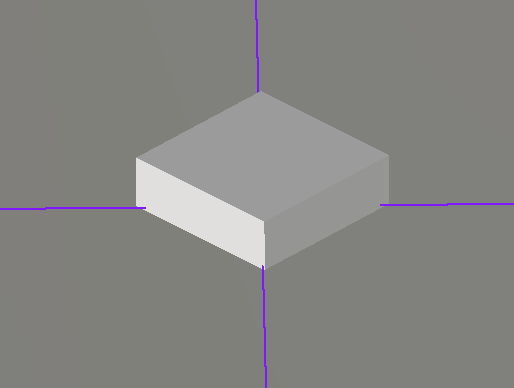
\includegraphics[width=1.00\textwidth]{figuras/Procedimiento_Simulaciones/Conduccion/modelado3D_centro_cerca.png}
		\caption{Vista cerca nano-espaciador}
		\label{fig:modelado3D_centro_cerca1}
	\end{subfigure}
	\caption{Vistas del sistema TPV. (\subref{fig:modelado3D_cerca}) Vista del sistema TPV de cerca desde un borde. (\subref{fig:modelado3D_centro_cerca}) Vista del nano-espaciador colocado sobre el centro de una cara de la célula.}
	\label{fig:modelado3D1}
\end{figure}
	\item Usar la herramienta \textbf{Active Model Assessment Tool}, que se encuentra en la pestaña de simulaciones, para generar el modelo de simulación de CFD\label{itm:pasoIniIterativo_Modelado3D1}.
	\item Guardar el modelo de CFD y volver al ensamblado de Inventor.
	\item Incrementar la altura del modelo del nano-espaciador un milímetro dentro del ensamblaje en Inventor, sin sobrepasar el máximo de 10 mm.
	\item Repetir todo 10 veces desde el paso \ref{itm:pasoIniIterativo_Modelado3D1}, teniendo como última iteración el modelo de la TPV con nano-espaciador de 10 mm, equivalente a 1 $\mu m$ de la realidad.
\end{enumerate} 

%%%%%%%%%%%%%%%%%%%%%%%%%%%%%%%%%%%%%%%%%%%
%   Procedimiento simulación CFD
\subsubsection{Procedimiento simulación CFD}
%%%  PROCEDIMIENTO CFD
El procedimiento a seguir para cada modelo de la simulación de transmisión de calor por conducción en CFD está detallado en el apéndice  \ref{ch:procedimientosSimCond}.\\\\ A continuación se expone un procedimiento sencillo sobre la realización de las simulaciones en CFD.
\begin{enumerate}
	\item Abrir el modelo o estudio correspondiente de simulación en CFD.
	\item Aplicar los materiales adecuados para cada componente con la propiedad de entorno puesta en \textit{variable}.
	\item Aplicar en caso que aplique la resistencia de contacto sobre la superficie superior del nano-espaciador.
	\item Aplicar las condiciones de contorno a los componentes del sistema, es decir, las temperaturas al emisor y a la célula.
	\item Aplicar un mallado apropiado para cada componente del sistema, teniendo el nano-espaciador una gran cantidad de nodos.
	\item Simular la transmisión de calor en el modo estacionario hasta llegar al régimen estacionario.
	\item Extraer o guardar los resultados de las potencias de conducción en un CSV.
	\item Repetir estos pasos para cada modelo con distintas alturas de nano-espaciadores.
\end{enumerate}